\section{Zhodnocení}
TODO

\subsection{Problémy}
Přestože model Boid vykazuje známky složitého chování, stále se řídí jednoduhými pravidly, které mohou zapříčinit nechtěné odchylky. Jednou z nich je tzv. semknutí dvou agentů, kteří se navzájem přetlačují a jeden druhému nedokáží ustoupit. To má za následek nechtěnné chování, které může zapříčinit, že tito agenti začnou procházet překážkami. 
\begin{figure}[H]
	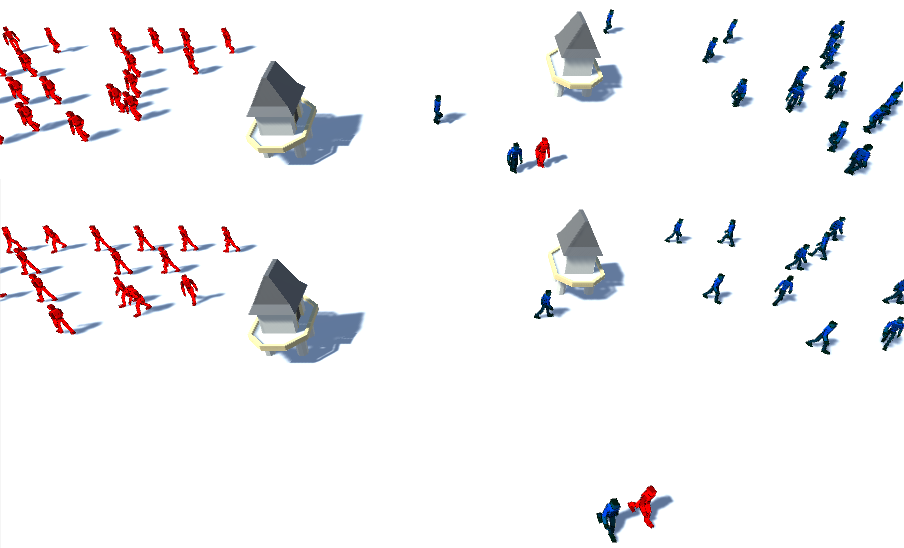
\includegraphics[width=10cm]{people_problem_anim.png}
	\centering
	\caption{Srážka a semknutí dvou agentů v časech $t\in\{ 100, 115\} $}
\end{figure}


